\chapter{Materias primas (Commodities)}\label{cap:commodities}

\section{Futuros: el instrumento}
Las materias primas se operan casi siempre con \textbf{futuros}: contratos estandarizados con
vencimiento, tamaño y entrega definidos. Lo que hay que conocer de cada contrato:
\begin{table}[h]\centering\small
\begin{tabular}{llllr}
\toprule
Símbolo & Contrato & Cotiza en & Multiplicador & Valor del tick \\ \midrule
CL & WTI (NYMEX) & \$/bbl & 1000 bbl & 10~\$ (0,01) \\
BZ & Brent (ICE) & \$/bbl & 1000 bbl & 10~\$ (0,01) \\
NG & Gas natural & \$/MMBtu & 10\,000 MMBtu & 10~\$ (0,001) \\
RB / HO & Gasolina / gasóleo & \$/gal & 42\,000 gal & 4,20~\$ (0,0001) \\
GC & Oro (COMEX) & \$/oz & 100 oz & 10~\$ (0,10) \\
SI & Plata & \$/oz & 5000 oz & 25~\$ (0,005) \\
HG & Cobre & \$/lb & 25\,000 lb & 12,50~\$ (0,0005) \\
ZC / ZS / ZW & Maíz / soja / trigo & ¢/bu & 5000 bu & 12,50~\$ (1/4 ¢) \\
\bottomrule
\end{tabular}
\caption{Especificaciones (\py{commodities.CONTRACTS}). Códigos de mes: F G H J K M N Q U V X Z = ene--dic.}
\end{table}

Un movimiento de 1~\$ en el crudo son 1000~\$ por contrato. Con un stop de 1,60~\$ y un riesgo de
1875~\$ solo cabe un contrato (\py{futures\_position\_size}); si no cabe ninguno, existen
micro-contratos (MCL, MGC) de 1/10.

\section{La curva de futuros}
El modelo de coste de mantenimiento (\emph{cost of carry}) relaciona contado y futuro:
\begin{equation}\label{eq:carry}
F(T) = S\,e^{(r+u-y)T},
\end{equation}
con $r$ el tipo de interés, $u$ el coste de almacenamiento y $y$ el \textbf{rendimiento de
conveniencia} (el valor de tener el físico disponible). Despejando,
$y = r+u-\ln(F/S)/T$ (\py{implied\_convenience\_yield}).
\begin{itemize}
\item \textbf{Contango} (curva creciente): inventarios abundantes, almacenaje caro. Típico de oro (casi
  puro coste financiero) y de gas en verano.
\item \textbf{Backwardation} (curva decreciente): escasez; el físico hoy vale más que mañana.
\end{itemize}

\section{Roll yield: por qué el precio no es la rentabilidad}
Quien mantiene exposición tiene que \emph{rodar} el contrato antes del vencimiento: vender el que vence
y comprar el siguiente. Si la curva no cambia, el contrato va «subiendo» o «bajando» por la curva hacia
el contado. El roll yield anualizado entre dos vencimientos es
\begin{equation}
RY = \frac{\ln(F_{\text{cerca}}/F_{\text{lejos}})}{T_{\text{lejos}}-T_{\text{cerca}}}
\end{equation}
(\py{commodities.roll\_yield}, \py{roll\_yield\_curve}): positivo en backwardation, negativo en contango.
\begin{figure}[h]\centering
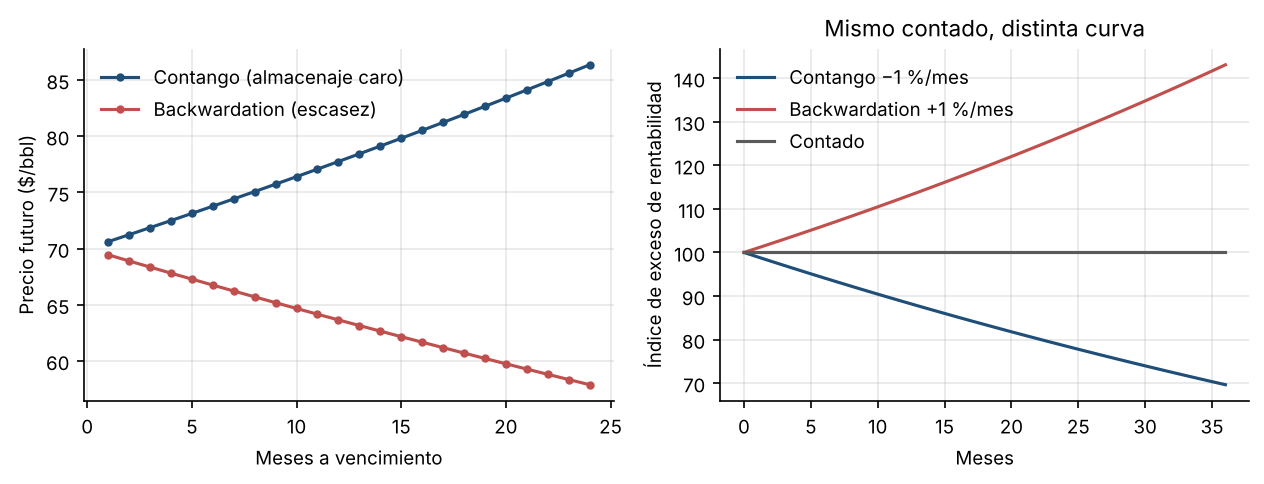
\includegraphics[width=\textwidth]{f09_curvas}
\caption{Izquierda: curvas en contango y backwardation. Derecha: con el mismo precio de contado, un
inversor que rueda gana o pierde un 1~\% mensual según la forma de la curva.}
\end{figure}
\begin{aviso}
Los ETF de materias primas que ruedan futuros en contango (gas natural, VIX) pierden valor de forma
sistemática aunque el contado no se mueva. Y las series «continuas» que enlazan contratos sin ajustar
tienen saltos falsos en cada roll: usa series ajustadas por ratio (\py{ratio\_back\_adjust}) para
backtests.
\end{aviso}

\paragraph{Carry como señal.} Estar largo en las materias primas con mayor backwardation y corto en las de
mayor contango (estrategia de \emph{carry} o de estructura de curva) es una de las primas más
documentadas del sector.

\section{Spreads}
Los traders de materias primas operan mucho más spreads que direcciones:
\begin{itemize}
\item \textbf{Calendario}: largo un vencimiento, corto otro (apuesta a la forma de la curva).
\item \textbf{Crack 3:2:1} (margen de refino, \$/bbl): $\big(2\cdot\text{RB}\cdot42+\text{HO}\cdot42-3\cdot\text{CL}\big)/3$ (\py{crack\_spread\_321}).
\item \textbf{Crush} de soja (\$/bu): harina$\times0{,}022$ + aceite$\times0{,}11$ $-$ soja (\py{crush\_spread}).
\item \textbf{Spark spread} (\$/MWh): electricidad $-$ heat rate $\times$ gas (\py{spark\_spread}).
\item \textbf{Inter-mercado}: Brent--WTI, oro/plata, trigo/maíz.
\end{itemize}

\section{Fundamentales y calendario}
\begin{itemize}
\item \textbf{Energía}: inventarios semanales EIA (miércoles, crudo; jueves, gas), reuniones de la OPEP+,
  huracanes, informes AIE. Margen de refino y estacionalidad (gasolina en verano, gasóleo en invierno).
\item \textbf{Metales preciosos}: tipos reales (el oro cae cuando suben los tipos reales a 10 años) y
  dólar; compras de bancos centrales; plata y platino con componente industrial.
\item \textbf{Metales industriales}: ciclo industrial y China (PMI), inventarios LME/SHFE.
\item \textbf{Agrícolas}: informes USDA (WASDE mensual, siembras de marzo, acreage de junio), clima,
  estacionalidad de cosecha (\py{monthly\_seasonality}).
\item \textbf{Posicionamiento}: informe COT de la CFTC (viernes): posiciones especulativas extremas
  anticipan giros.
\end{itemize}

\begin{practica}
Nunca mantengas un futuro con entrega física hasta el primer día de aviso (\emph{first notice day})
si no puedes recibir el físico: rueda antes. El 20 de abril de 2020 el WTI de mayo cotizó a $-37$~\$
porque los compradores sin almacenaje no podían recibir el crudo.
\end{practica}

\begin{ejercicios}
\begin{enumerate}
\item Precios CL 78,1 / 77,4 / 76,9 / 76,5 para 1--4 meses: forma de la curva y roll yield
  (\py{python scripts/calculadoras.py curva --precios ... --meses 1 2 3 4}).
\item Crudo 75~\$, RBOB 2,35~\$/gal, HO 2,55~\$/gal: calcula el crack 3:2:1.
\item Con oro a 2400~\$, tipo 4,5~\% y futuro a 6 meses a 2460~\$, ¿qué rendimiento de conveniencia
  implícito hay (con $u=0$)?
\end{enumerate}
\end{ejercicios}
